\documentclass[tikz,border=20pt]{standalone}
\usepackage{helvet}
\renewcommand{\familydefault}{\sfdefault}
\usetikzlibrary{positioning, arrows.meta, decorations.markings, calc, fit}
\usepackage{pagecolor}

\definecolor{navyblue}{HTML}{0F172A}
\definecolor{copper}{HTML}{B87333}

\begin{document}
\pagecolor{white}
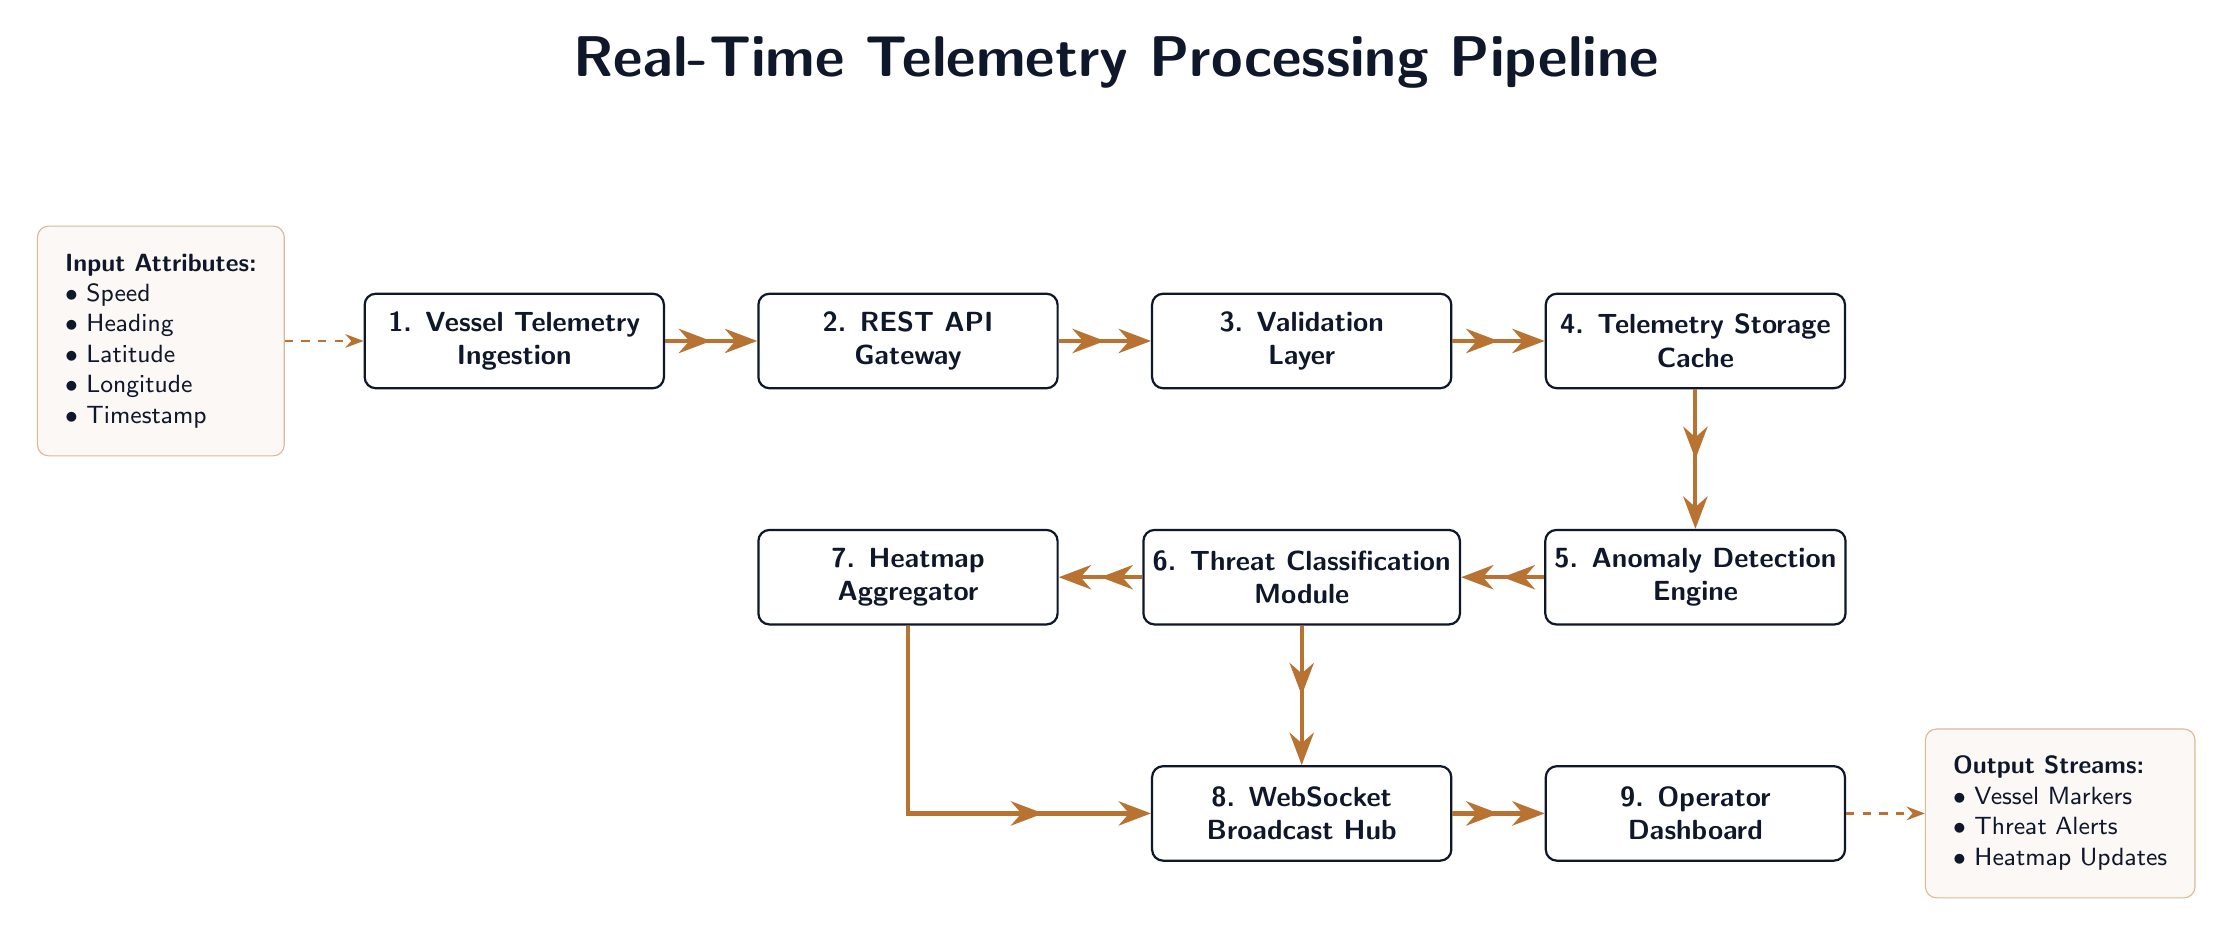
\begin{tikzpicture}[
    font=\sffamily,
    box/.style={rectangle, draw=navyblue, thick, fill=white, rounded corners, minimum width=3.8cm, minimum height=1.2cm, align=center, text=navyblue, font=\bfseries},
    annot/.style={rectangle, draw=copper!50, fill=copper!5, rounded corners, align=left, font=\small\color{navyblue}, inner sep=10pt},
    streamarrow/.style={
        copper, line width=1.5pt,
        postaction={decorate, decoration={
            markings,
            mark=at position 0.5 with {\arrow{Stealth[scale=1.2]}}
        }},
        -{Stealth[scale=1.2]}
    },
    streamarrow_ortho/.style={
        copper, line width=1.5pt,
        postaction={decorate, decoration={
            markings,
            mark=at position 0.75 with {\arrow{Stealth[scale=1.2]}}
        }},
        -{Stealth[scale=1.2]}
    }
]

% ==================== NODES ====================
\node[box] (ingest) at (0, 0) {1. Vessel Telemetry\\Ingestion};
\node[box] (gateway) at (5, 0) {2. REST API\\Gateway};
\node[box] (validation) at (10, 0) {3. Validation\\Layer};
\node[box] (cache) at (15, 0) {4. Telemetry Storage\\Cache};

\node[box] (anomaly) at (15, -3) {5. Anomaly Detection\\Engine};
\node[box] (classification) at (10, -3) {6. Threat Classification\\Module};
\node[box] (heatmap) at (5, -3) {7. Heatmap\\Aggregator};

\node[box] (hub) at (10, -6) {8. WebSocket\\Broadcast Hub};
\node[box] (dashboard) at (15, -6) {9. Operator\\Dashboard};

% ==================== ANNOTATIONS ====================
\node[annot, left=1cm of ingest] (input_annot) {
    \textbf{Input Attributes:}\\
    $\bullet$ Speed\\
    $\bullet$ Heading\\
    $\bullet$ Latitude\\
    $\bullet$ Longitude\\
    $\bullet$ Timestamp
};

\node[annot, right=1cm of dashboard] (output_annot) {
    \textbf{Output Streams:}\\
    $\bullet$ Vessel Markers\\
    $\bullet$ Threat Alerts\\
    $\bullet$ Heatmap Updates
};

% ==================== CONNECTING ANNOTATIONS ====================
\draw[copper, dashed, thick, -{Stealth}] (input_annot.east) -- (ingest.west);
\draw[copper, dashed, thick, -{Stealth}] (dashboard.east) -- (output_annot.west);

% ==================== CONTINUOUS STREAM ARROWS ====================
% Row 1: Forward
\draw[streamarrow] (ingest.east) -- (gateway.west);
\draw[streamarrow] (gateway.east) -- (validation.west);
\draw[streamarrow] (validation.east) -- (cache.west);

% Row 1 to Row 2: Down
\draw[streamarrow] (cache.south) -- (anomaly.north);

% Row 2: Backward
\draw[streamarrow] (anomaly.west) -- (classification.east);
\draw[streamarrow] (classification.west) -- (heatmap.east);

% Row 2 to Row 3: Hub Convergence
\draw[streamarrow] (classification.south) -- (hub.north);
\draw[streamarrow_ortho] (heatmap.south) |- (hub.west);

% Row 3: Forward
\draw[streamarrow] (hub.east) -- (dashboard.west);

% ==================== TITLE ====================
\node[fit=(input_annot) (cache) (dashboard) (output_annot)] (bounding) {};
\node[above=1.5cm of bounding.north, font=\huge\bfseries\color{navyblue}] {Real-Time Telemetry Processing Pipeline};

\end{tikzpicture}
\end{document}
